%! TeX root = ../main.tex
\chapter{METODOLOGI}
\label{chap:metodologi}

% Ubah bagian ini sesuai dengan metodologi penelitian proposal / tugas akhir Anda.

\section{Diagram Alir Penelitian}
\label{sec:diagramalir}

Metodologi penelitian ini dilakukan melalui tahapan sebagaimana ditunjukkan pada Gambar~\ref{fig:alir-metodologi}. \lipsum[1]

\begin{figure}[H]
  \centering
  % Ganti berkas gambar berikut dengan diagram alir penelitian Anda di folder gambar/
  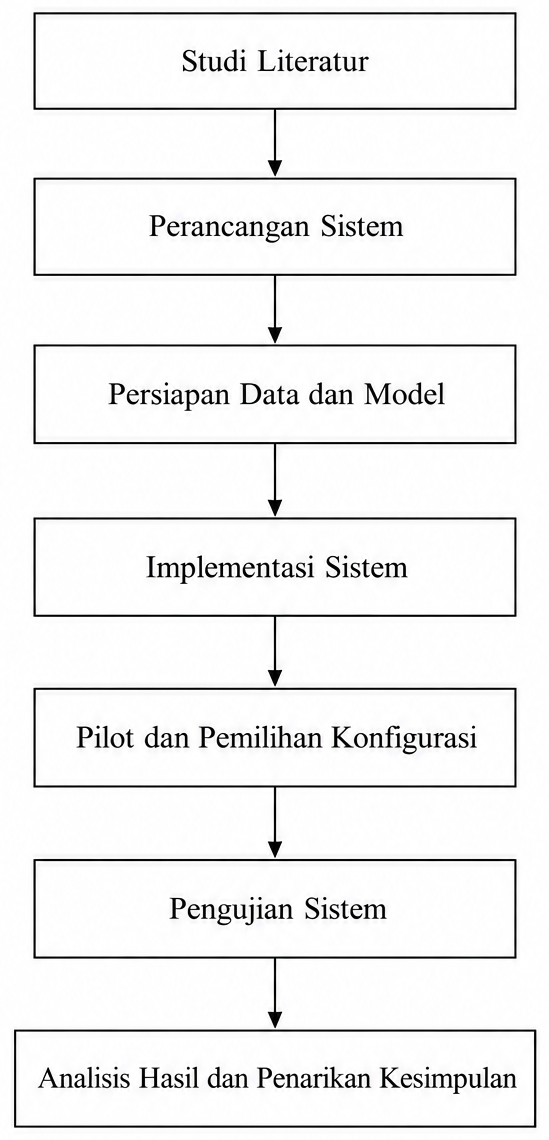
\includegraphics[height=12cm]{gambar/gambar-3-1.png}
  \caption{Diagram Alir Metodologi Penelitian}
  \label{fig:alir-metodologi}
\end{figure}

\section{Bahan dan Peralatan}
\label{sec:bahanperalatan}

Pada bagian ini diuraikan bahan, spesifikasi peralatan, perangkat keras (\emph{hardware}), dan perangkat lunak (\emph{software}) yang digunakan dalam penelitian.

\lipsum[2]

\begin{enumerate}
  \item \textbf{Perangkat Keras}: \lipsum[3][1-2]
  \item \textbf{Perangkat Lunak}: \lipsum[4][1-2]
\end{enumerate}

\section{Perancangan Sistem}
\label{sec:perancangansistem}

\subsection{Arsitektur dan Diagram Blok Sistem}
\label{subsec:arsitektursistem}

Sistem dirancang dengan alur kerja yang menghubungkan setiap modul dari akuisisi data, prapemrosesan, pemrosesan utama, hingga keluaran atau tampilan antarmuka. Hubungan antarblok sistem dan aliran data ditunjukkan pada Gambar~\ref{fig:blok-sistem}.

\begin{figure}[H]
  \centering
  % Ganti berkas gambar berikut dengan diagram blok sistem Anda di folder gambar/
  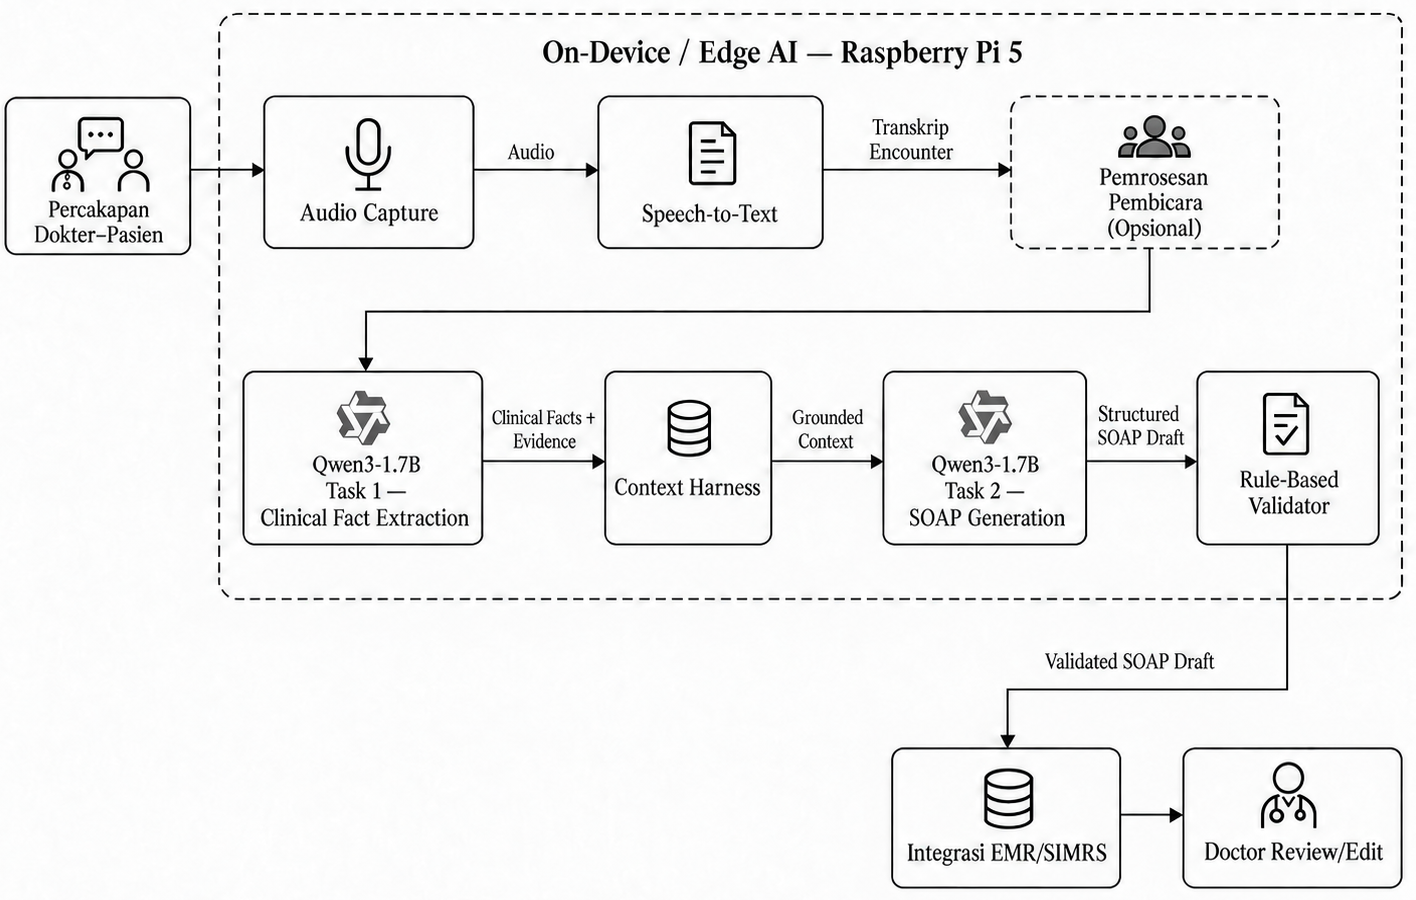
\includegraphics[width=0.9\textwidth]{gambar/gambar-3-2.png}
  \caption{Diagram Blok Sistem}
  \label{fig:blok-sistem}
\end{figure}

\subsection{Tahapan Implementasi}
\label{subsec:tahapanimplementasi}

\lipsum[5-6]

\section{Prosedur Pengujian dan Evaluasi}
\label{sec:pengujiandanevaluasi}

Bagian ini menjelaskan skenario pengujian, parameter atau metrik evaluasi yang diamati, serta metode analisis data yang digunakan untuk menjawab rumusan masalah.

\lipsum[7-8]

\section{Jadwal Kegiatan}
\label{sec:jadwalkegiatan}

Rincian pelaksanaan kegiatan penelitian tugas akhir disajikan pada Tabel~\ref{tab:jadwalkegiatan}.

\begin{table}[htbp]
  \centering
  \caption{Jadwal Kegiatan Pelaksanaan Tugas Akhir}
  \label{tab:jadwalkegiatan}
  \begin{tabularx}{\textwidth}{|c|X|c|c|c|c|}
    \hline
    \textbf{No} & \textbf{Nama Kegiatan} & \textbf{Bulan 1} & \textbf{Bulan 2} & \textbf{Bulan 3} & \textbf{Bulan 4} \\
    \hline
    1 & Studi Literatur dan Perumusan Masalah & $\bullet$ & & & \\
    \hline
    2 & Perancangan dan Implementasi Sistem & & $\bullet$ & $\bullet$ & \\
    \hline
    3 & Pengujian Fungsional dan Evaluasi & & & $\bullet$ & $\bullet$ \\
    \hline
    4 & Analisis Data dan Penyusunan Laporan & & & & $\bullet$ \\
    \hline
  \end{tabularx}
\end{table}
